\documentclass[11pt]{article}
\usepackage[margin=1in]{geometry}
\usepackage{amsmath,amssymb}
\usepackage{graphicx}
\usepackage{booktabs}
\usepackage[hidelinks]{hyperref}
\usepackage{siunitx}
\graphicspath{{figs/}}

\title{Physical $W$-shape for the $\phi$ diffractive generator:\\
fixing the near-threshold cross section from photoproduction}
\author{Valery Kubarovsky (with Claude)}
\date{2026-07-01}

\begin{document}
\maketitle

\begin{abstract}
The tuned $\phi$ electroproduction cross section used a threshold factor
$(1-W_{th}^2/W^2)^{\alpha_2}$ with a \emph{negative} exponent
($\alpha_2=-1.245$), which diverges at threshold -- unphysical, and it blows
up the radiative-correction (RC) integral. We show that CLAS12 data cannot
constrain the near-threshold $W$-shape, fix that shape to real-photon
photoproduction (Roberts et al., Eq.~23b: $\alpha_2=2$, $\alpha_3=\epsilon=0.20$),
and refit only the two parameters CLAS12 does constrain -- the $t$-slope $b_t$
and the $Q^2$ exponent $\nu_T$. The result describes the data equally well
($\chi^2=13.0$ vs $11.3$), is physical at threshold, and makes the RC
well-behaved (bounded $\eta$, no blow-ups).
\end{abstract}

\section{The problem}

The $\phi$ generator models the transverse cross section as
\begin{equation}
\frac{d\sigma_T}{dt} = \alpha_1
\left(1-\frac{W_{th}^2}{W^2}\right)^{\alpha_2}\!W^{\alpha_3}
\left(1+\frac{Q^2}{m_\phi^2}\right)^{-\nu_T}\!b_t\,e^{b_t t},
\qquad
\frac{d\sigma_L}{dt}=c_R\frac{Q^2}{m_\phi^2}\frac{d\sigma_T}{dt},
\label{eq:model}
\end{equation}
with $W_{th}=m_p+m_\phi=1.96$~GeV. The original tuning returned
$\alpha_2=-1.245$. A \emph{negative} threshold exponent makes
$(1-W_{th}^2/W^2)^{\alpha_2}\to\infty$ as $W\to W_{th}$: the cross section
\emph{diverges} at threshold instead of vanishing (Fig.~\ref{fig:problem}).
This is unphysical, and it is fatal for the radiative correction: the RC
integral samples $\sigma_T$ at the radiatively-shifted
$W'=\sqrt{W^2-v}<W$, which is dragged toward $W_{th}$, so the integrand
explodes. In an independent RC scan ($60$-point grid) the old model gave
$\eta=\sigma_{obs}/\sigma_{Born}$ up to $13$ with MC variance as large as the
value, at $\sim1/3$ of grid points.

\begin{figure}[h]\centering
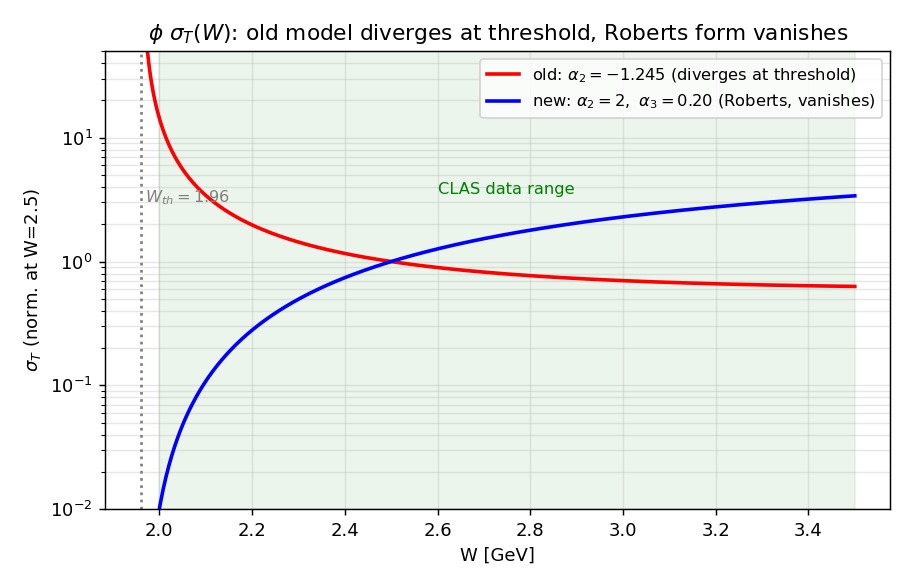
\includegraphics[width=0.72\textwidth]{sigmaW_problem}
\caption{$\phi$ $\sigma_T(W)$ near threshold (log scale, normalised at
$W=2.5$). The old model ($\alpha_2=-1.245$, red) diverges as $W\to W_{th}$;
the Roberts form ($\alpha_2=2$, $\alpha_3=0.20$, blue) vanishes at threshold
and rises with $W$ as the Pomeron dictates. The CLAS data live in the shaded
band, $\sim40$~MeV above threshold.}
\label{fig:problem}
\end{figure}

\section{Why CLAS12 cannot fix the $W$-shape}

The CLAS12 $\phi$ data span $W\in[2.0,3.5]$~GeV -- the lower edge is only
$\sim40$~MeV above threshold, and $W$ is strongly correlated with $Q^2$ in
fixed-target electroproduction. Consequently the $W$-shape is essentially
unconstrained: fitting $\alpha_2,\alpha_3$ freely gives per-dataset
$\alpha_3$ scattered over $0.22$--$1.44$ (a factor $6$), and the fit exploits
the \emph{negative} $\alpha_2$ merely as an extra in-range shape knob with no
physical meaning. Forcing $\alpha_2\ge0$ while still \emph{fitting} $\alpha_3$
does not help: $\alpha_2$ pins to $0$, $\alpha_3$ swings to $\approx-3$, and
$\chi^2$ triples ($11\to32$). The data simply do not know the $W$-shape.

\section{The fix: take the $W$-shape from photoproduction}

Real-photon photoproduction \emph{does} measure the $W$-shape, over a wide
clean range. Roberts et al.\ (arXiv:2510.08845) parametrise the total cross
section with the all-$W$ Donnachie--Landshoff form (their Eq.~23b),
\begin{equation}
\sigma(W)=\sigma_{\mathbb P}\left[1-\frac{(m_p+m_V)^2}{W^2}\right]^{2}W^{\epsilon},
\label{eq:23b}
\end{equation}
which is \emph{identical in structure} to the $W$-part of
Eq.~\eqref{eq:model}. For $\phi$ their P-dyn fit gives $\epsilon=0.20$. We
therefore fix
\begin{equation}
\boxed{\ \alpha_2=2\quad(\text{threshold, }\sigma_T\to0),\qquad
\alpha_3=\epsilon=0.20\quad(\text{Roberts P-dyn }\phi)\ }
\end{equation}
and fit only $b_t$ and $\nu_T$ to CLAS12. The normalisation $\alpha_1$ stays a
free scale (the tuning fits shapes, not absolute normalisation);
$c_R=1$ fixed. The exponent $2$ is the DL convention -- what physics requires
is only that it be positive (phase space gives $\ge1/2$); the value does not
affect the CLAS fit because $b_t,\nu_T$ are orthogonal to the $W$-shape.

\section{The fit}

For each of the five CLAS12 RGA datasets we generate $\phi$ MC with the fixed
$W$-shape, apply the neural-network fast simulation for acceptance, extract
the $\phi$ signal by fitting $M(K^+K^-)$ in each kinematic bin
(Fig.~\ref{fig:mkk}), acceptance-correct the data, and fit $b_t,\nu_T$ to the
corrected $W,Q^2,t$ distributions (Figs.~\ref{fig:accept},
\ref{fig:fitdetail}). Only $b_t$ and $\nu_T$ are free.

\begin{figure}[h]\centering
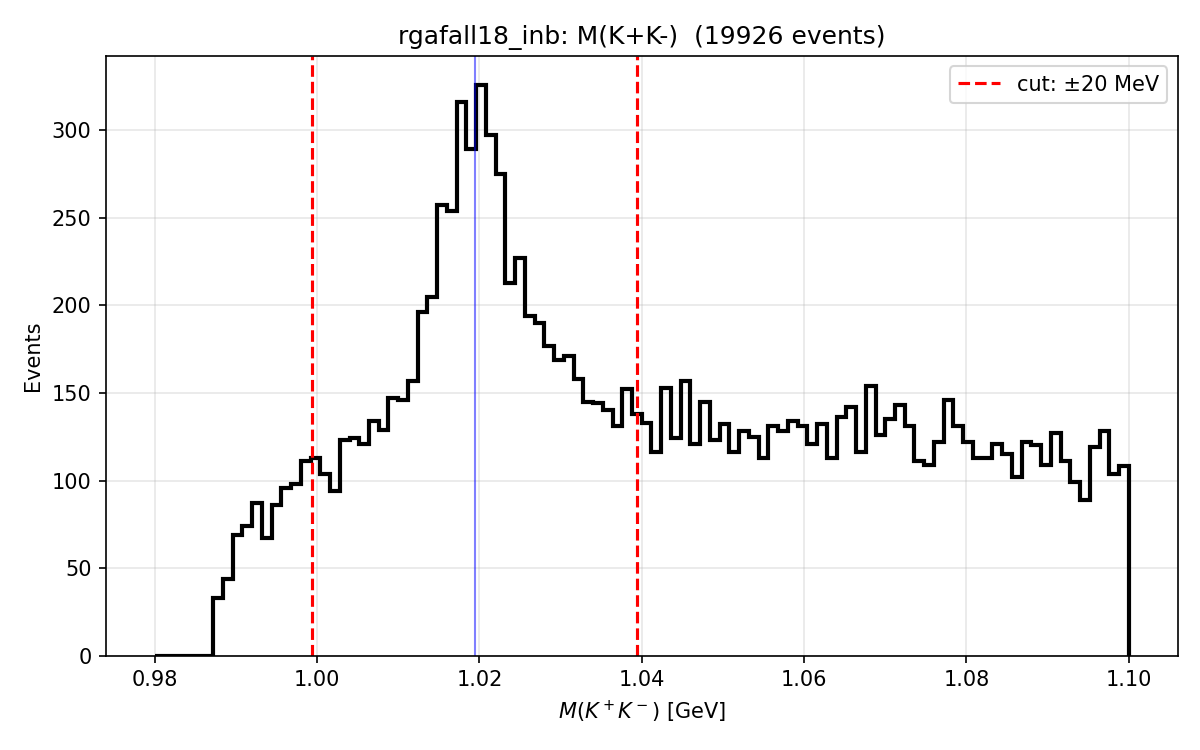
\includegraphics[width=0.49\textwidth]{mkk_data_fall18inb}
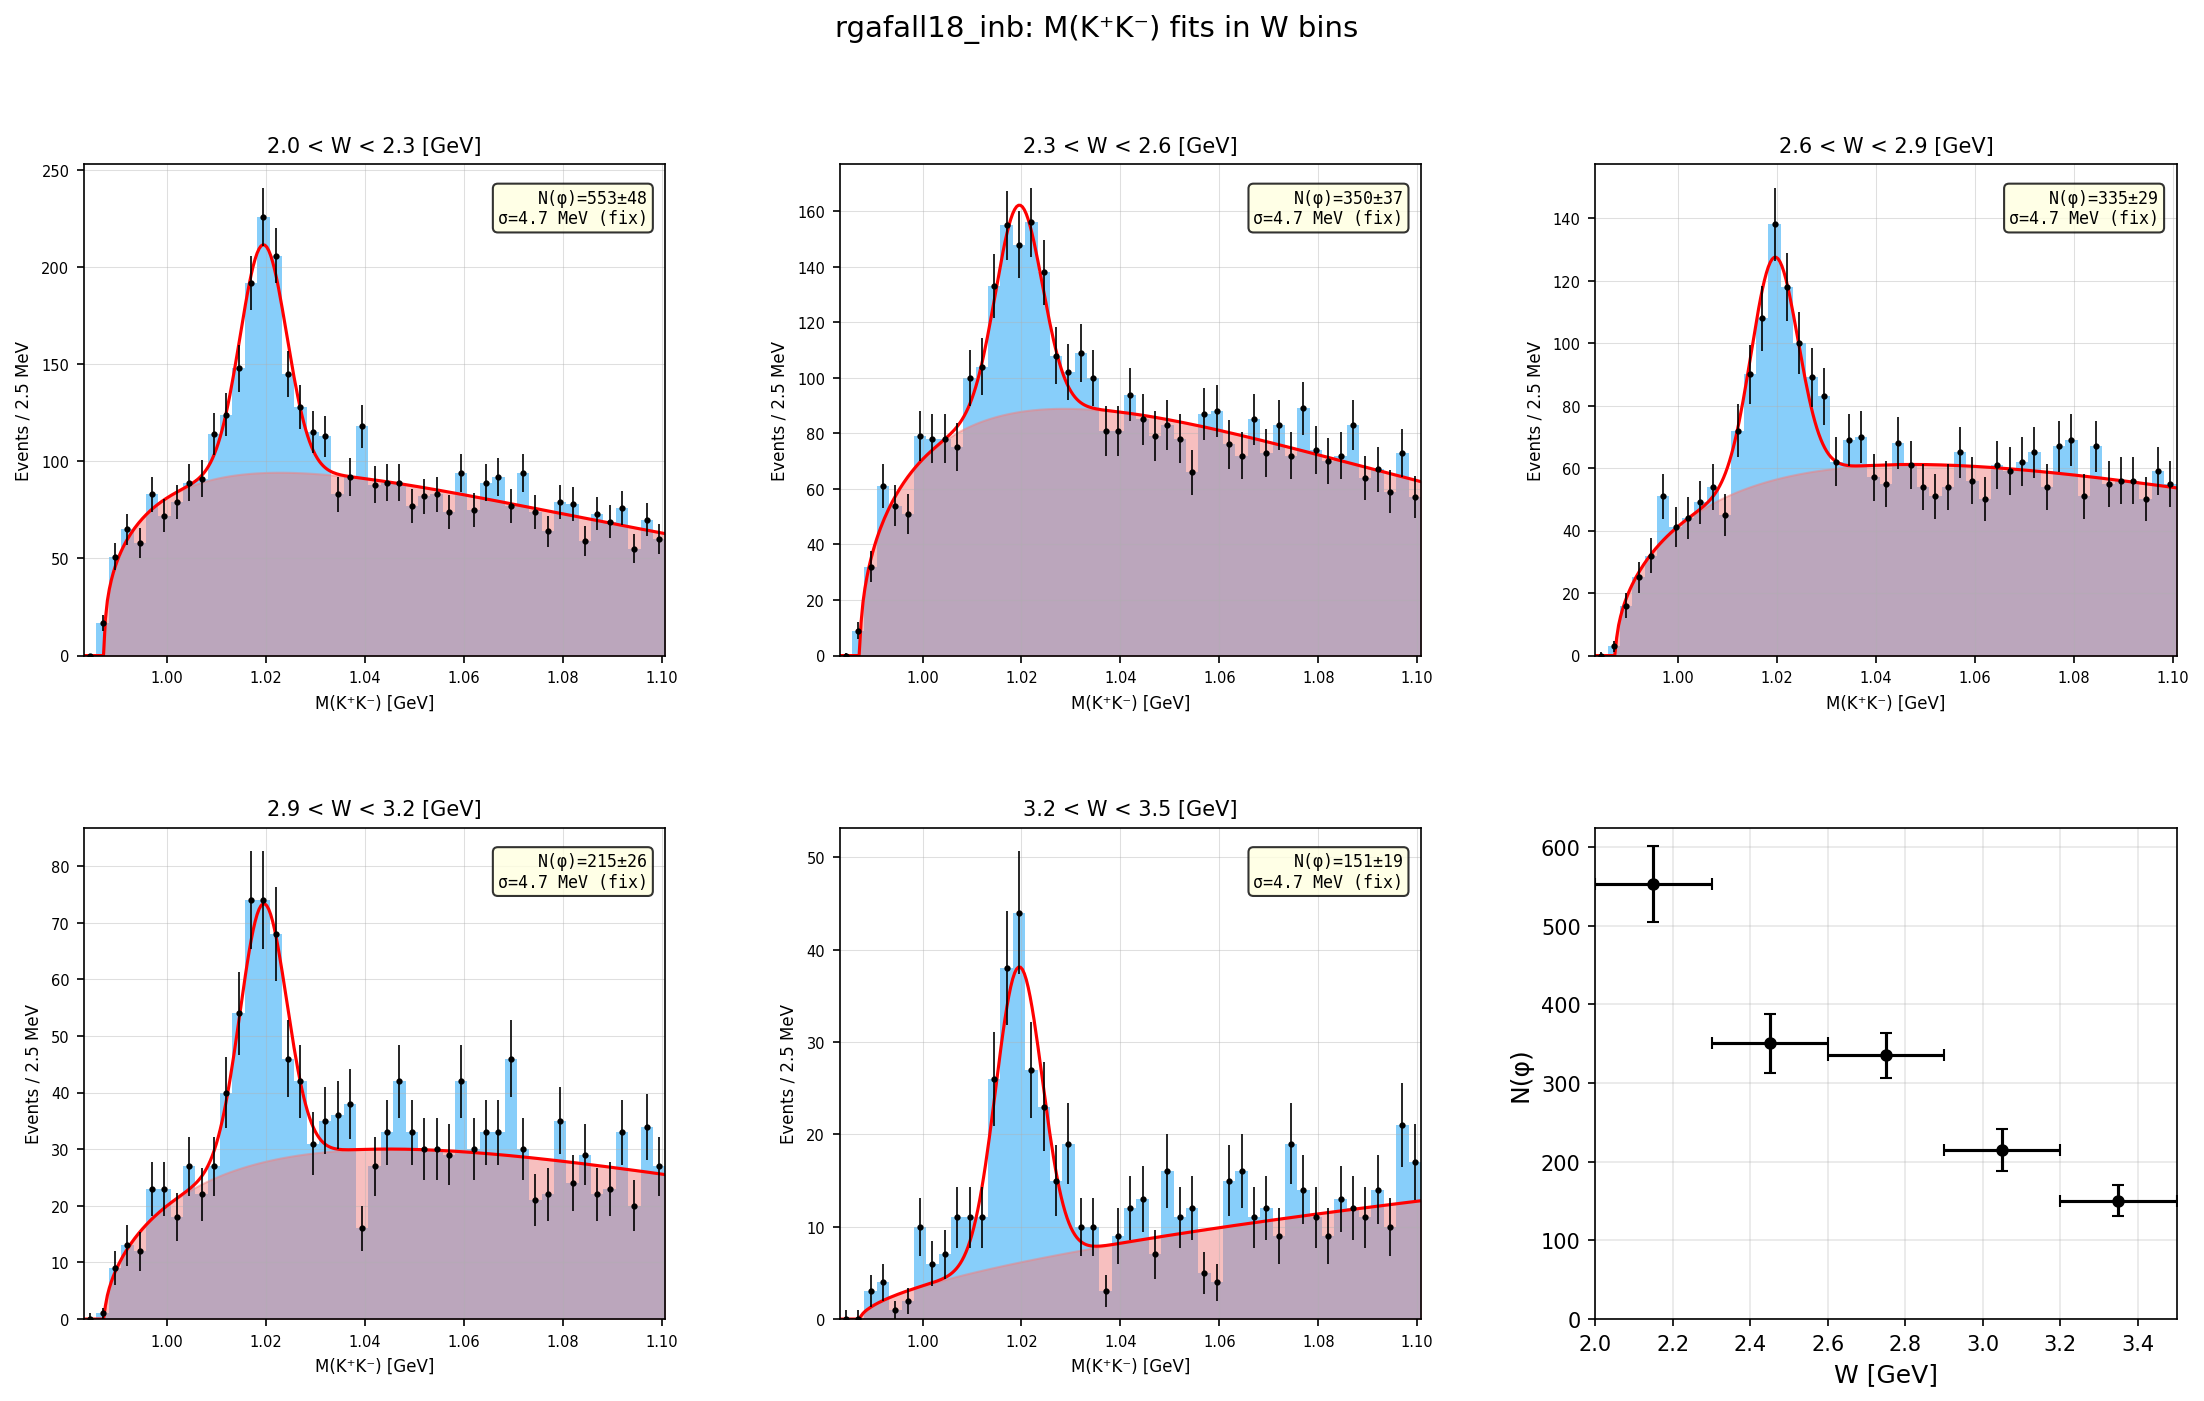
\includegraphics[width=0.49\textwidth]{mkk_binned_w_fall18inb}
\caption{Signal extraction (Fall18-inb). Left: inclusive $M(K^+K^-)$ with the
$\phi$ peak. Right: the $\phi$ yield from fitting $M(K^+K^-)$ in bins of $W$.}
\label{fig:mkk}
\end{figure}

\begin{figure}[h]\centering
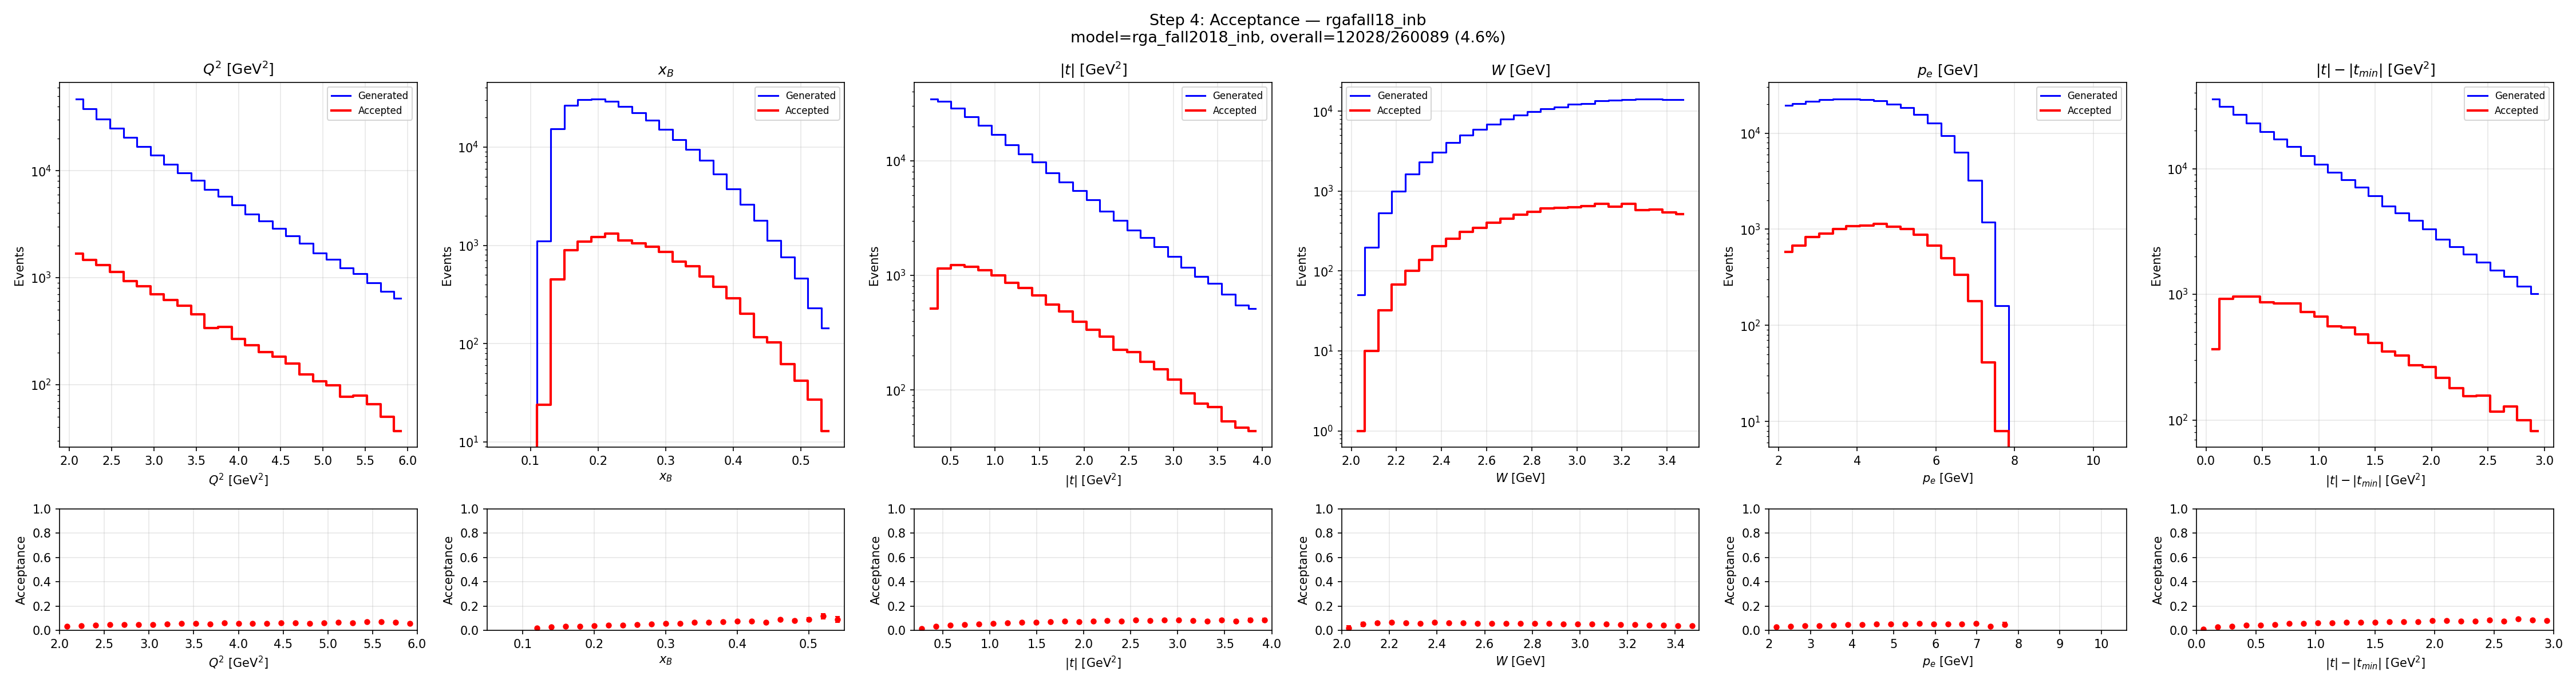
\includegraphics[width=0.75\textwidth]{acceptance_fall18inb}
\caption{Acceptance from the NN fast simulation vs.\ $W,Q^2,t,x_B$
(Fall18-inb).}
\label{fig:accept}
\end{figure}

\begin{table}[h]\centering
\caption{Final $\phi$ fit. $\alpha_2=2$, $\alpha_3=0.20$ fixed (Roberts
Eq.~23b, P-dyn); $c_R=1$; $\alpha_1$ free. Only $b_t,\nu_T$ fit.}
\begin{tabular}{lccc}
\toprule
dataset & $b_t$ [GeV$^{-2}$] & $\nu_T$ & $\chi^2$ \\
\midrule
Fall18 inb  & 1.248 & 2.327 & 14.9 \\
Fall18 outb & 1.470 & 2.557 & 18.4 \\
Sp18 inb    & 1.348 & 2.072 &  9.6 \\
Sp18 outb   & 1.321 & 2.237 & 11.8 \\
Sp19 inb    & 1.245 & 2.074 & 10.2 \\
\midrule
\textbf{average} & \textbf{1.326$\pm$0.082} & \textbf{2.253$\pm$0.181} & \textbf{13.0} \\
\bottomrule
\end{tabular}
\label{tab:fit}
\end{table}

The result (Table~\ref{tab:fit}) has $\chi^2=13.0$, statistically identical to
the old free fit ($11.3$), with $b_t,\nu_T$ essentially unchanged and now
\emph{tighter}. The negative-$\alpha_3$ pathology is gone: because we no longer
ask the data to set the $W$-shape, there is nothing to force $\alpha_3$
negative.

\begin{figure}[h]\centering
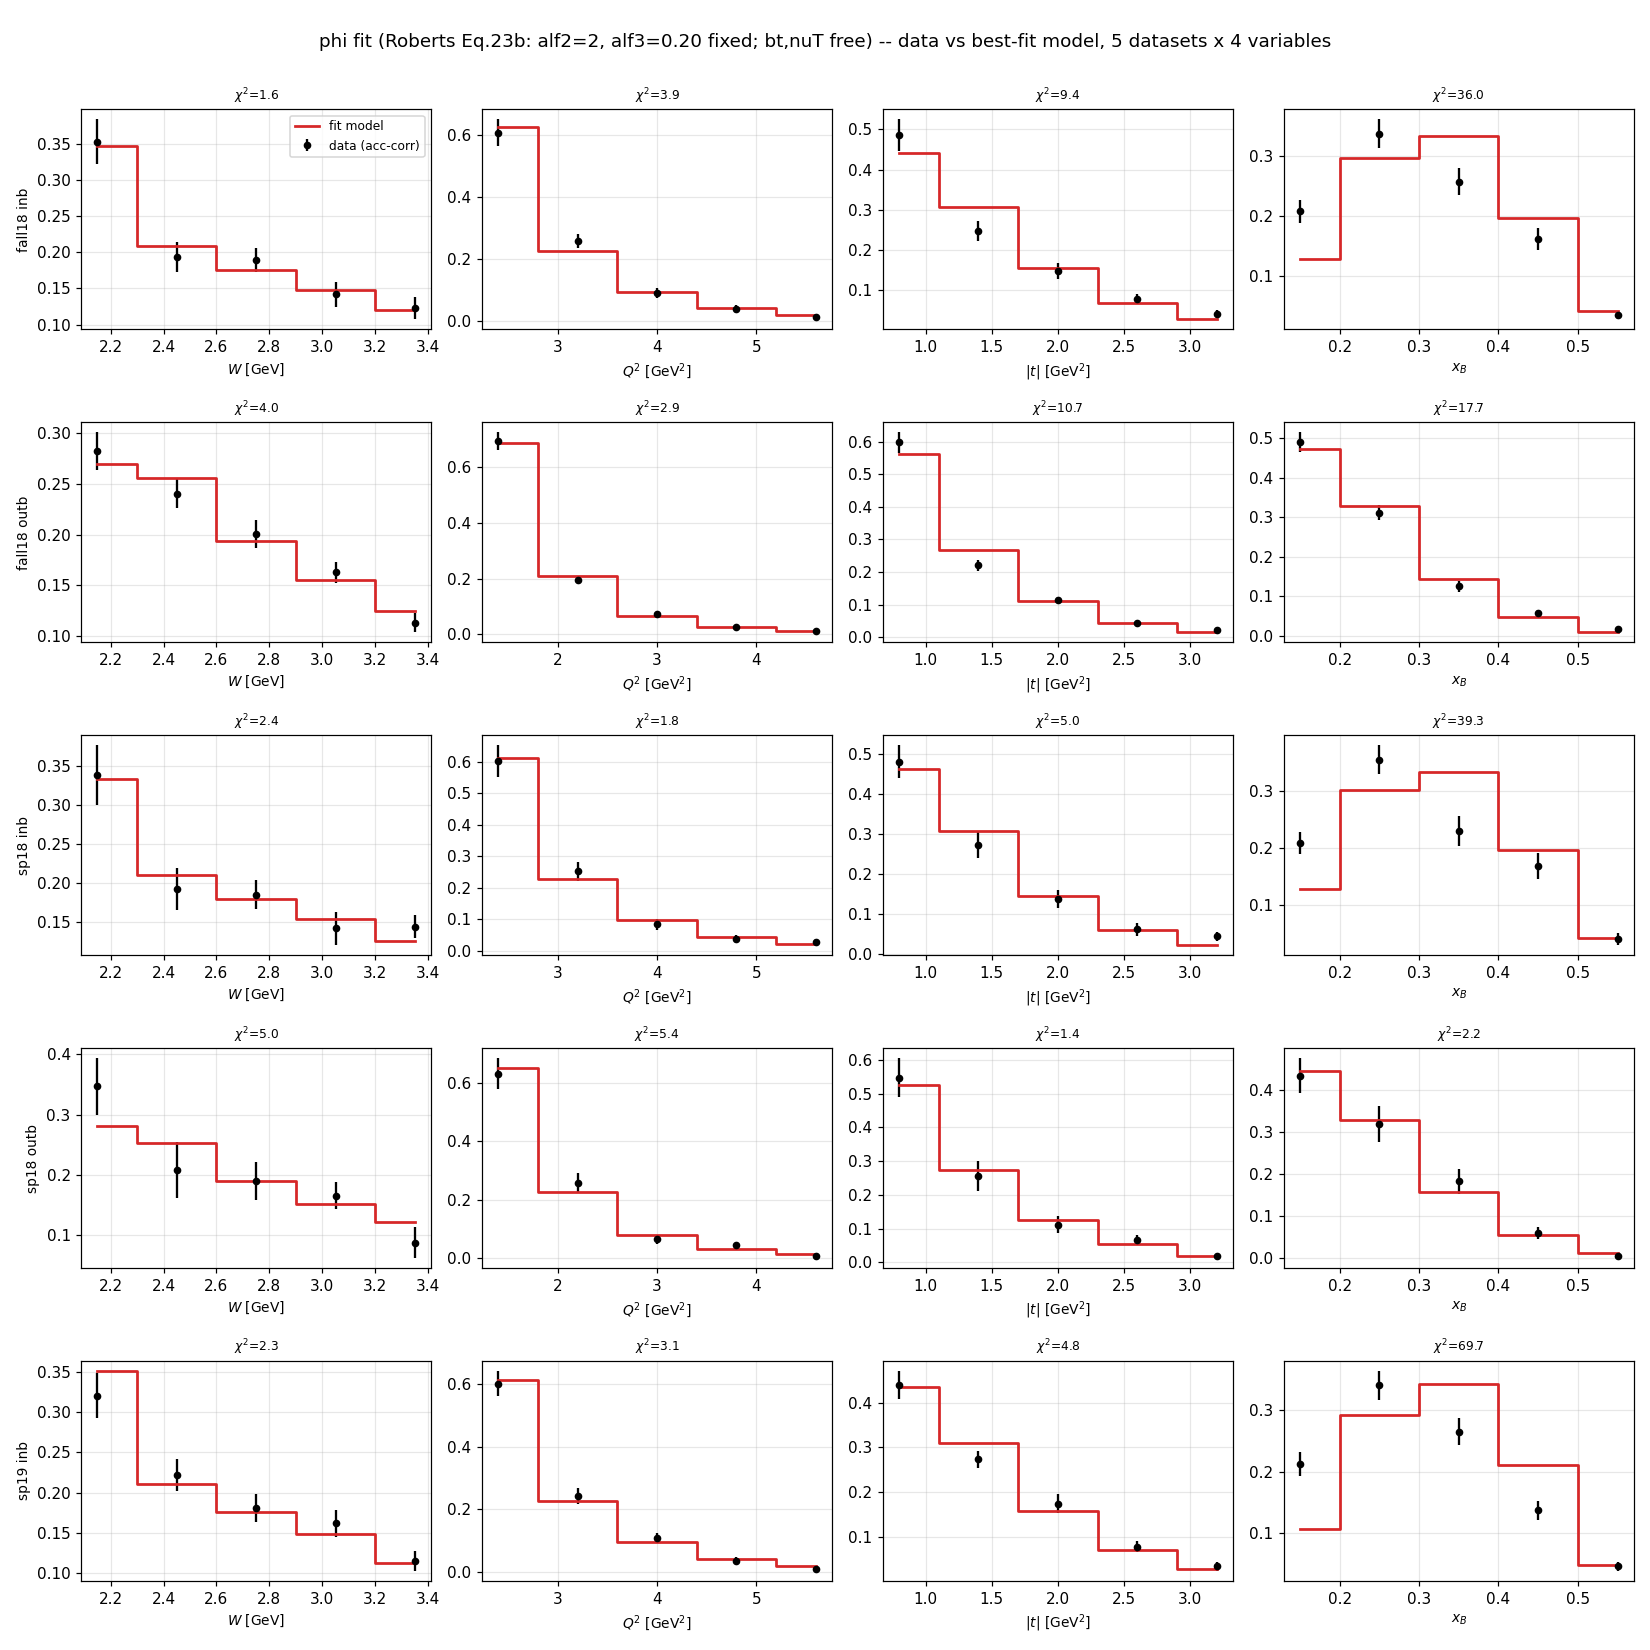
\includegraphics[width=\textwidth]{fit_all}
\caption{Acceptance-corrected data (black) vs.\ best-fit model (red) for all
five datasets $\times$ four variables ($W,Q^2,|t|,x_B$). $\chi^2$ per panel
shown; the fit uses $W,Q^2,t$.}
\label{fig:fitall}
\end{figure}

\begin{figure}[h]\centering
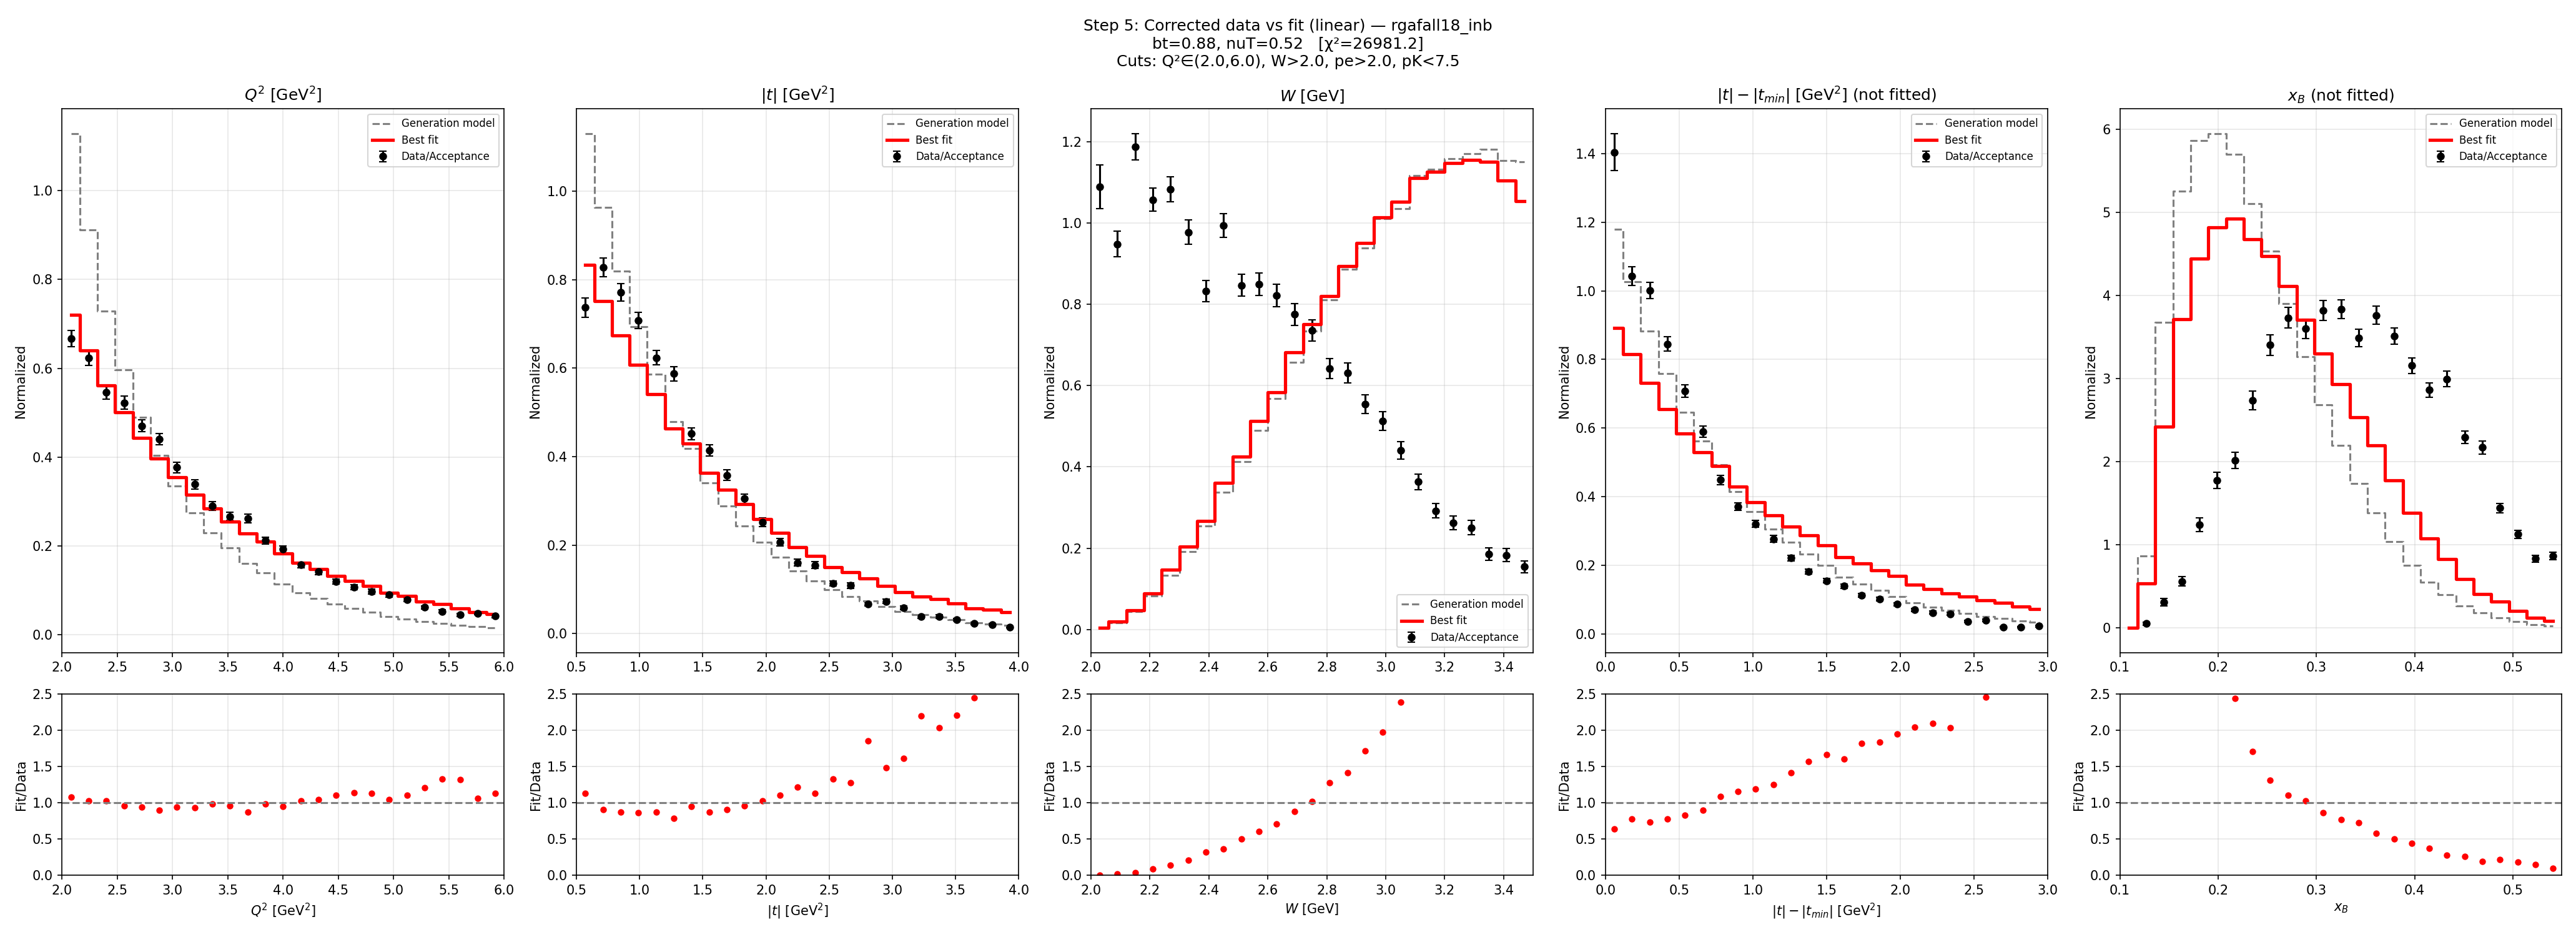
\includegraphics[width=0.9\textwidth]{fit_detail_fall18inb}
\caption{Data vs.\ best-fit model, Fall18-inb (detail).}
\label{fig:fitdetail}
\end{figure}

\paragraph{Note on iteration.} The standard tuning iterates
generate$\to$refit. With the $W$-shape fixed, that loop does \emph{not}
converge: $\chi^2$ stays flat at $13.0$ while $b_t,\nu_T$ drift and the
inter-dataset spread grows (an unstable regenerate--refit map along a flat
$b_t$--$\nu_T$ valley). A single reweighting pass already recovers the answer;
iteration is unnecessary and destabilising here. The single-pass values in
Table~\ref{tab:fit} are the result.

\section{Radiative-correction verification}

Re-running the RC $60$-point grid with the new $W$-shape confirms the fix:
$\eta$ is bounded to $0.745$--$0.840$ with \textbf{0/60 blow-ups}
(Fig.~\ref{fig:rc}), versus $19/60$ diverging points for the old model. The
model dependence of the RC is small ($\sim6\%$ in the diffractive region;
Fig.~\ref{fig:rc}, right).

\begin{figure}[h]\centering
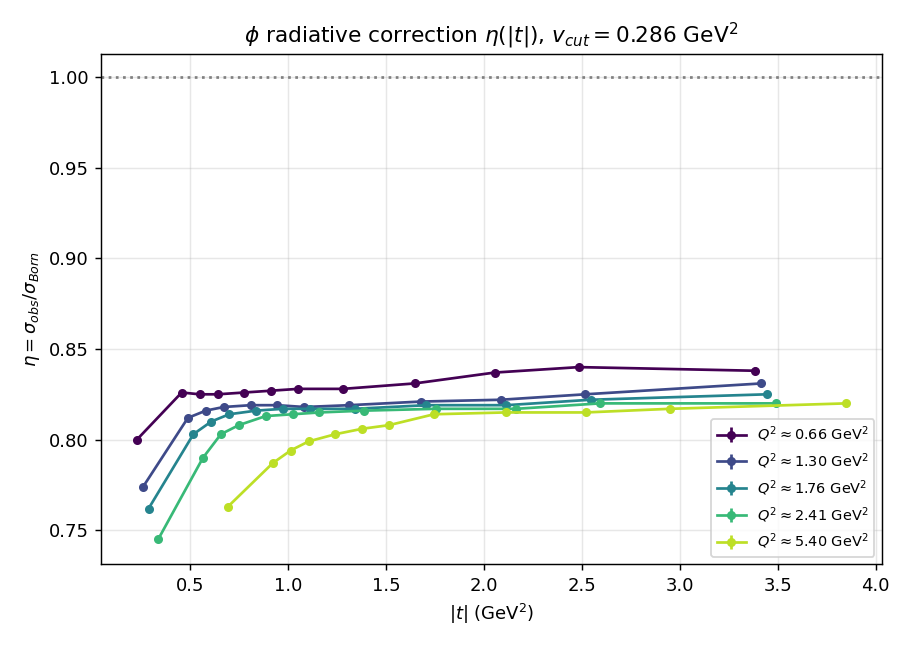
\includegraphics[width=0.49\textwidth]{rc_eta_roberts}
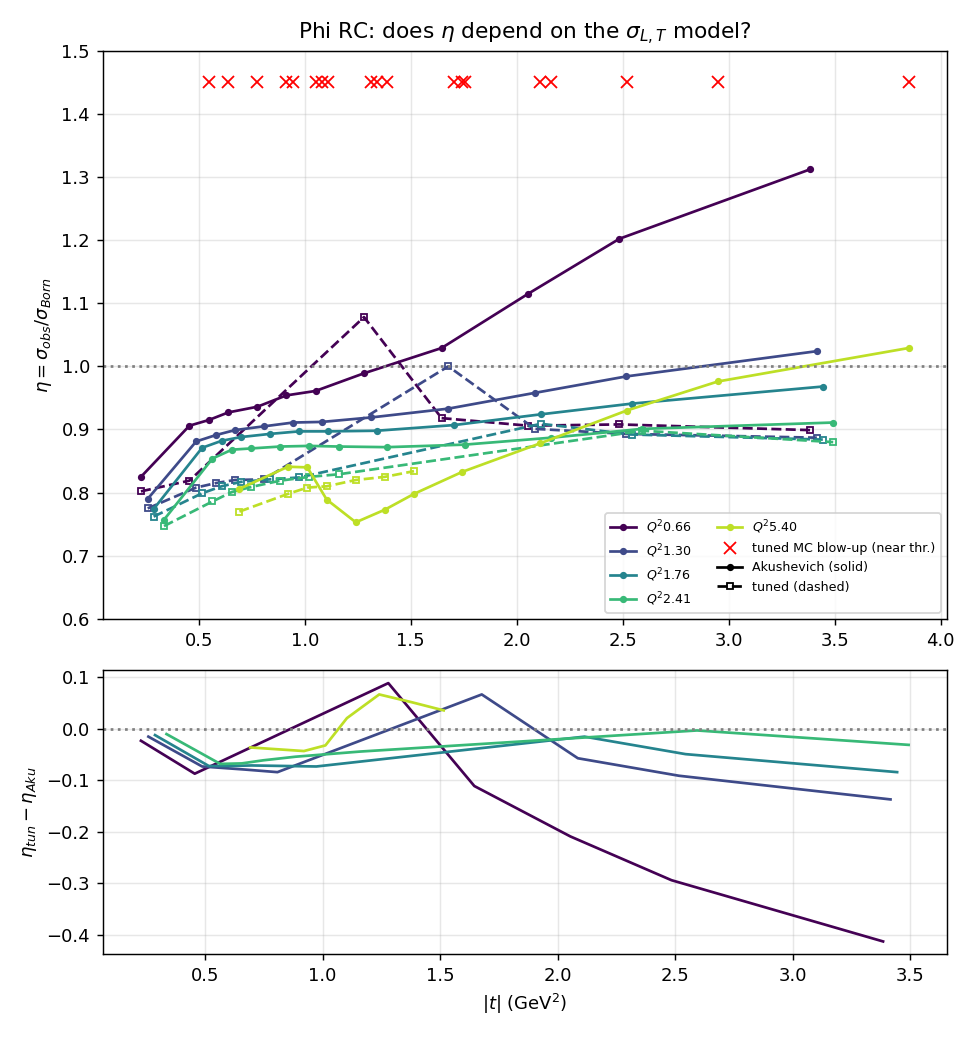
\includegraphics[width=0.49\textwidth]{eta_model_compare}
\caption{Left: RC factor $\eta(|t|)$ with the Roberts $W$-shape -- smooth,
bounded, physical. Right: $\eta$ model comparison (Akushevich vs.\ tuned),
$\sim6\%$ in the diffractive region.}
\label{fig:rc}
\end{figure}

\section{Where the parameters live (three directories)}

The final $\phi$ parameters are used in three separate code bases. They must be
kept consistent; if the $\phi$ tuning is ever redone, \emph{all three} must be
updated together.

\begin{table}[h]\centering
\caption{The final $\phi$ cross-section parameters and where they are set.
Averaged values: $\alpha_2=2$, $\alpha_3=0.20$, $b_t=1.326$, $\nu_T=2.253$,
$c_R=1$, $\alpha_1$ free.}
\small
\begin{tabular}{lll}
\toprule
Directory & File (function) & Role \\
\midrule
\texttt{vector\_mesons\_generator\_tuning} & \texttt{phi/diffrad\_vpk\_exp.f90}
& tuning generator \\
 & \quad + \texttt{phi/runs/*/config.json} & (determines params) \\
\texttt{MC\_vector\_mesons} & \texttt{diffrad\_vm.f90} (\texttt{sigma\_T\_phi})
& production / RC generator \\
\texttt{RC\_vector\_mesons\_DIFFRAD} &
\texttt{tuned\_roberts\_phi\_run/mdiffrad.f} (\texttt{difflt}) &
RC $\eta$-grid calculation \\
\bottomrule
\end{tabular}
\label{tab:dirs}
\end{table}

All three now carry $\alpha_2=2$, $\alpha_3=0.20$, $\nu_T=2.253$, $b_t=1.326$,
$c_R=1$. In \texttt{diffrad\_vm.f90} and the tuning generator these are the
compiled defaults (overridable by input-file keys
\texttt{alf1 alf2 alf3 nuT bt cR}); in \texttt{difflt} they are hard-coded in
the \texttt{ivec=3} branch.

\section{Summary}

\begin{itemize}
\item The old $\phi$ $W$-shape ($\alpha_2=-1.245$) was unphysical (diverges at
threshold) and broke the RC.
\item CLAS12 cannot determine the near-threshold $W$-shape.
\item Fixing it to photoproduction (Roberts Eq.~23b P-dyn:
$\alpha_2=2,\ \alpha_3=0.20$) and fitting only $b_t=1.326\pm0.082$,
$\nu_T=2.253\pm0.181$ describes the data equally well ($\chi^2=13.0$), is
physical at threshold, and makes the RC bounded.
\item Free parameters: $b_t,\nu_T$ (fit); $\alpha_1$ (free normalisation).
Fixed: $\alpha_2,\alpha_3$ (photoproduction), $c_R$.
\end{itemize}

\end{document}
